The majority of signals searched for using ECAL time reconstruction involve "prompt" signals. Prompt signals are the result of a stable particle that interacts with the detectors that are produced with no significant displacement, or delay, from the time and location of the primary interaction (PV). There is a rich field of study involving searches for signals that are not prompt. These "delayed" signals often result when a semi-stable particle, often called a long lived particle ( LLP ), is produced and travels a significant distance from the PV, often at $\beta < 1$, before it decays resulting in the production of stable particles that are then seen in the detectors. The total time it takes for the LLP to decay plus the time for the resultant stable particles to travel to the detectors is typically larger than the time it would take for a stable particle to travel from the PV directly to the detectors. Such signals are said to have "large delay times". The performance of the CC algorithm was studied with simulated samples where large delay times are expected due to the presence of LLPs. 
%presence of LLPs using the HTo2LongLivedTo4b Monte Carlo ( MC ) datasets. These datasets were produced to study the use of timing information for the L1 trigger in Run 3 with $\sqrt{s} = 14$ TeV and are motivated by neutral naturalness models in which a Higgs decays to two LLPs that in turn decay to two Bs. Since the LLP's decay at a significantly displaced distance from the primary vertex, the hadronization of the resulting Bs into jets will be significantly delayed from the time of the interactions at the primary vertex and will occur at a displaced secondary vertex. The combination flight time of the LLP to its displaced decay vertex plus the subsequent jets' flight time from the displaced vertex to the face of the ECAL will have a minimum possible value equal to that of the prompt time flight time  from the PV and typically be much larger. Therefore the jets resulting from the hadronization of the Bs will tend to have significantly delayed arrival times at the face of the ECAL when compared to those arising from typical prompt interactions. To simulate a range of delay times, the simulated events where produced for Higgs masses of 1000, 350, 250, and 125 GeV that decay to a range of possible LLP masses for selected LLP life times ($\tau$) ranging from $c\tau =$ 100000 mm to $c\tau =$ 500 mm. To characterize the performance of CC algorithm is samples with large delay times, the central value and the resolution of the reconstructed times were studied.

In order to study the accuracy of the reconstructed time it is necessary to compare the reconstructed time to a "true", or truth, time. A truth time for each reconstructed time is determined using the record of the amount and time of the energy deposits in each ECAL crystal present in the MC dataset, called pCaloHits.  This truth time, or gen-time, for a rechit is calculated from the energy weighted average of the pCaliHit times used to simulate the pulse from which the rechit time is reconstructed.
 
\hfill
\begin{figure}[h!tbp]
\begin{center}
\resizebox{0.45\textwidth}{!}{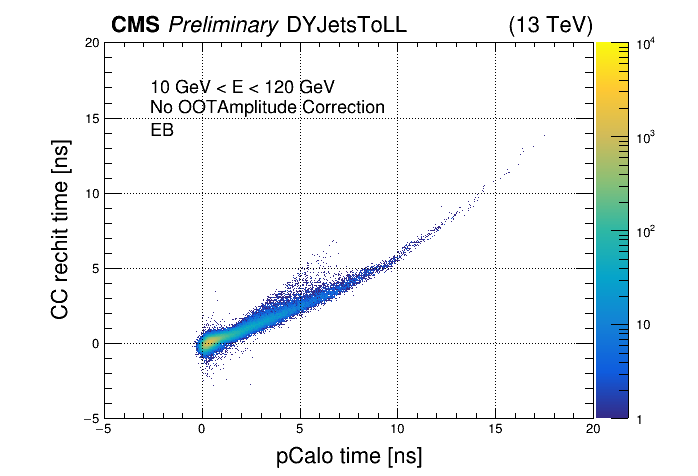
\includegraphics{fig/sec_gen/tr_2d_PCvCC_delay_13062022150058.png}}
\resizebox{0.45\textwidth}{!}{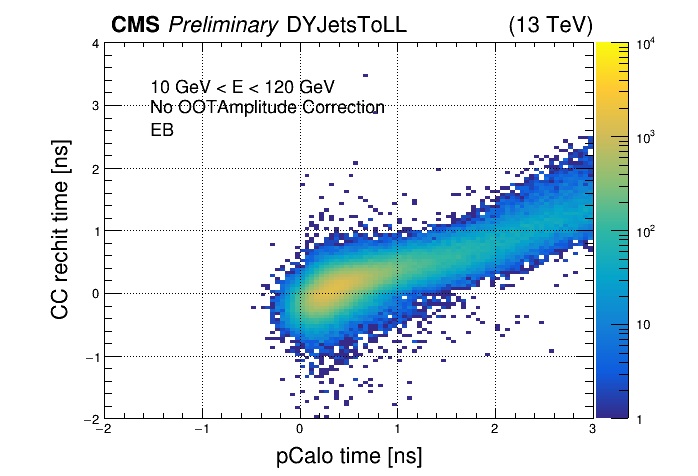
\includegraphics{fig/sec_gen/tr_2d_PCvCC_delay_zoom_13062022150920.png}}
%\resizebox{0.35\textwidth}{!}{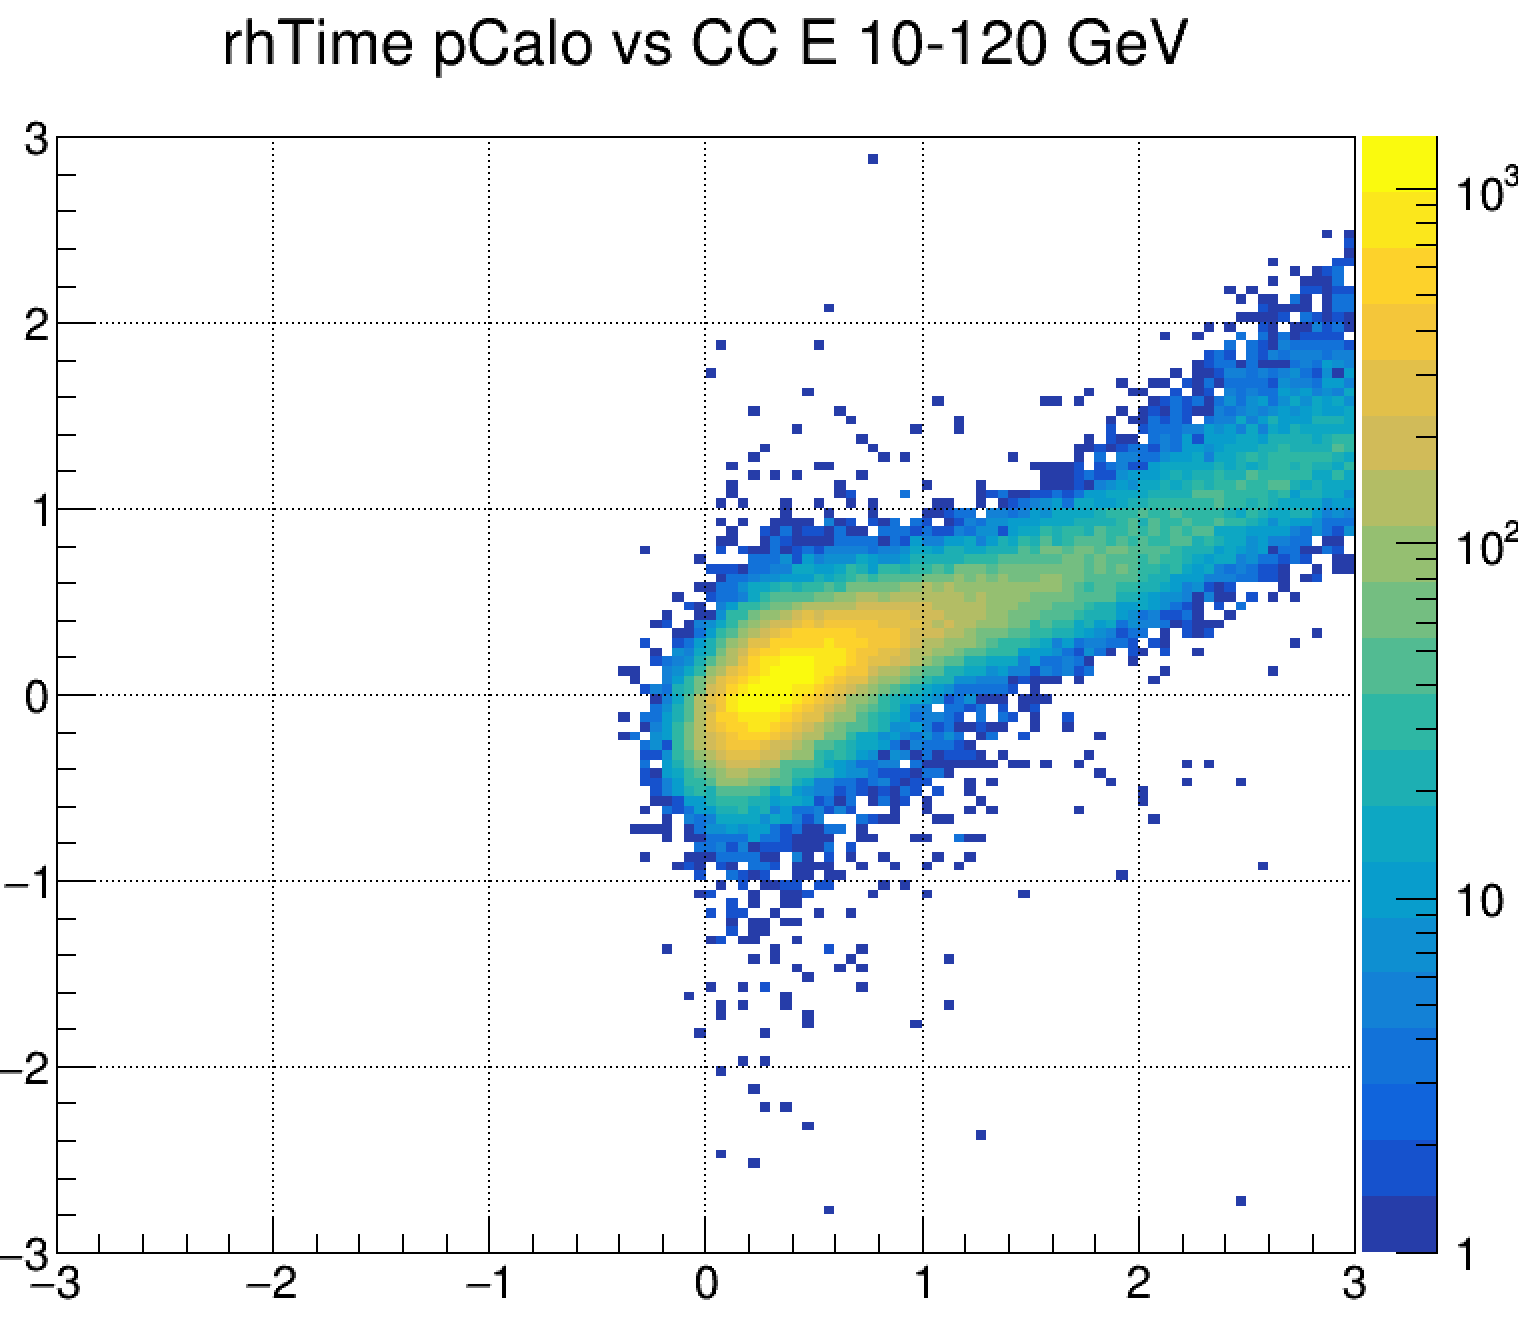
\includegraphics{fig/sec_gen/pc_v_cc_baised_zoom.png}}
\caption{The gen-time for each rechit is plotted with respect to the rechit time produced by the CC algorithm in the HTo2LongLivedTo4b Monte Carlo dataset. The gen-time is the energy weighted average of the gen-time associated with a particular rechit. The CC rechit time has no calibration applied. In the plot on the left a significant bias is shown in the reconstruction for times delayed more than $\sim$1 ns. In the plot on the right, the scale is expanded to examine the performance of the KUCC algorithm for times less than $\sim$1 ns, where it is seen that there is very good agreement with the gen-time.}
\label{pc_v_cc_bais}
\end{center}
\end{figure}

In Figure~\ref{pc_v_cc_bais} the gen-time for each rechit was determined and plotted against the rechit time produced by the CC algorithm. In the plot on the left of this figure a significant bias is shown in the reconstruction for times delayed more than $\sim$1 ns. In the right hand plot in this figure, the scale is expanded to examine the performance of the CC algorithm for times less than $\sim$1 ns. At this scale it is seen that there is very good agreement between the CC reconstruction and the gen-times for prompt signals.

\hfill
\begin{figure}[h!tbp]
\begin{center}
\resizebox{0.7\textwidth}{!}{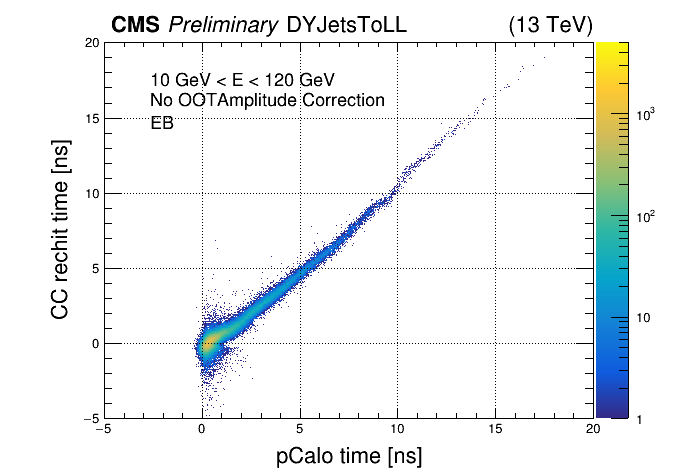
\includegraphics{fig/sec_gen/tr_2d_PCvCC_delay_nocorr_09062022175333.png}}
\caption{The gen-time for each rechit is plotted with respect to the rechit time produced by the CC algorithm, with the OOT amplitude corrections turned off in the time reconstruction. The CC rechit time has no calibration applied. Here we see that when the OOT amplitude corrections in the CC algorithm are disabled there is no bias at large delay times in the time reconstruction.}
\label{pc_v_cc_nooot}
\end{center}
\end{figure}

In Figure~\ref{pc_v_cc_nooot} the time reconstructed by a modified CC algorithm is plotted with respect to the gen-time. In this modified version of the CC algorithm, the OOT amplitude corrections to the pulse shape are not applied. In this plot no bias is observed at for large delay times, thereby demonstrating that the bias in the CC reconstruction is introduced by the OOT amplitude corrections. As discussed in Section \ref{sec:algo2}, the OOT amplitude correction step utilizes the OOT amplitudes produced by the multifit algorithm to remove the contributions of OOT pulses in the measured pulse in order to recover the "in-time" pulse.  When the OOT amplitudes are determined in the multifit algorithm, it is assumed that the OOT amplitudes occur at fixed times. Since OOT contributions to the pulse shape do not occur at fixed times, this introduces a bias in the OOT amplitudes.  

%This bias in the OOT amplitudes can be seen in the energy reconstruction. In Figure~\ref{ootamp_bias_multi} the arrival time of a jet ( Jet Time ) is plotted against the ratio of the reconstructed jet energy to the associated "true" jet energy. The jet time is found by taking the resolution weighted mean of the rechit times of all rechits within a dR of 0.3 of the jet, where the time reconstruction used is the default ratio method. As is demonstrated in Figure~\ref{ootamp_bias_multi}, there is a significant bias in the jet energy at large delay times. 

To account for this bias the CC algorithm reconstructs the rechit time with and without the OOT amplitude correction. The time with the OOT amplitude correction is used for the time of the rechit. The difference between the time with and without the OOT amplitude correction is found and preserved.  While the uncorrected CC times do not benefit from OOT-PU mitigation, the unbiased times are of interest for an analysis involving LLPs.  The time reconstructed without the OOT amplitude correction can be by utilizing a dedicated function in the ECAL rechit collection of the CMS analysis framework ( CMSSW ).

%To account for this bias the CC algorithm checks the reconstructed time produced with the OOT amplitudes corrections and if the time exceeds a particular threshold, typically X ns, the reconstruction is performed with the the OOT amplitude corrections turned off. The correlation of the delay time bias aware KUCC algorithm with the pCalo gen time is shown in Figure~\ref{pc_v_cc_fixed}.

%\hfill
%\begin{figure}[h!tbp]
%\begin{center}
%\resizebox{0.7\textwidth}{!}{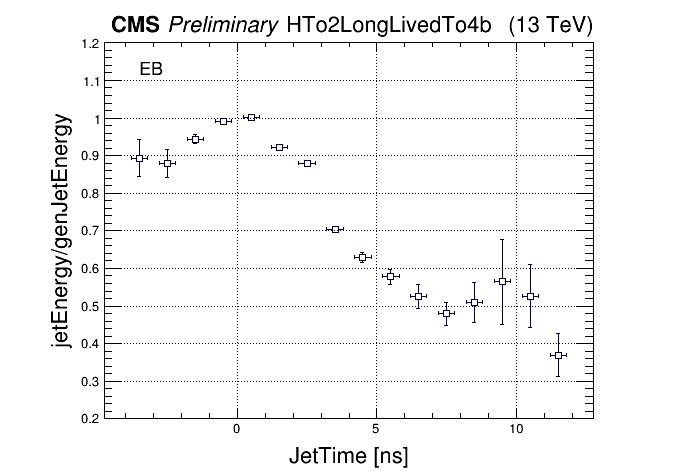
\includegraphics{fig/sec_gen/tr_hl_HTo2LongLivedTo4b_eratio_09062022173703.png}}
%\caption{The arrival time of a jet is plotted with respect to the ratio of the jet energy to the associated gen jet energy in the HTo2LongLivedTo4b Monte Carlo dataset. The jet time is found by taking the resolution weighted mean of the rechit times of all rechits with dR $<$ 0.3 of the jet. The ratio time reconstruction method is used for the rechit time. Here the effect of assuming that the OOT amplitudes occurs at fixed times is seen in the bias of the energy reconstruction at large delay times.}
%\label{ootamp_bias_multi}
%\end{center}
%\end{figure}

%In Figure~\ref{cc_delay_res} the impact on the resolution of forgoing the OOT amplitude corrections in the CC time reconstruction is studied. In this plot the Same RO unit resolution is plotted as per the method outlined in Section~\ref{sec:resmeth1} for the ratio algorithm, the KUCC algorithm, and the KUCC algorithm without OOT amplitude corrections. As can be seen, the resolution for the KUCC algorithm without OOT amplitude corrections is significantly degraded compared to the KUCC algorithm with OOT amplitude corrections, as is to be expected. The performance of the KUCC algorithm without OOT amplitude corrections is still improved when compared to the ratio method. %When the reconstruction is preformed in data without the OOT amplitudes for a specified threshold value there is a marginal degradation in the resolution as shown in Figure~\ref{cc_delay_res}.

%\hfill
%\begin{figure}[h!tbp]
%\begin{center}
%\resizebox{0.75\textwidth}{!}{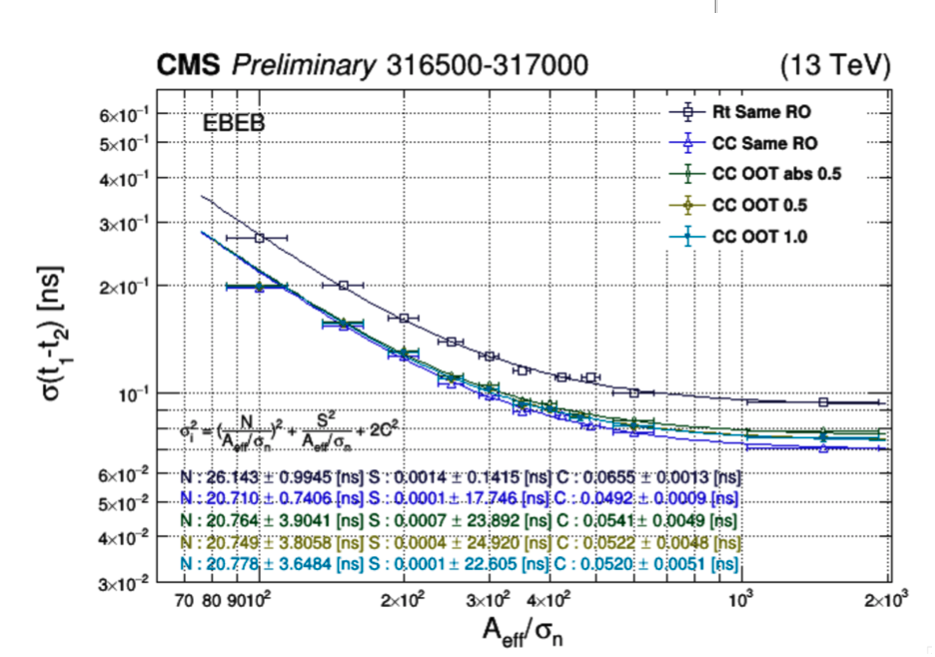
\includegraphics{fig/sec_gen/delayed_cc_res.png}}
%\resizebox{0.7\textwidth}{!}{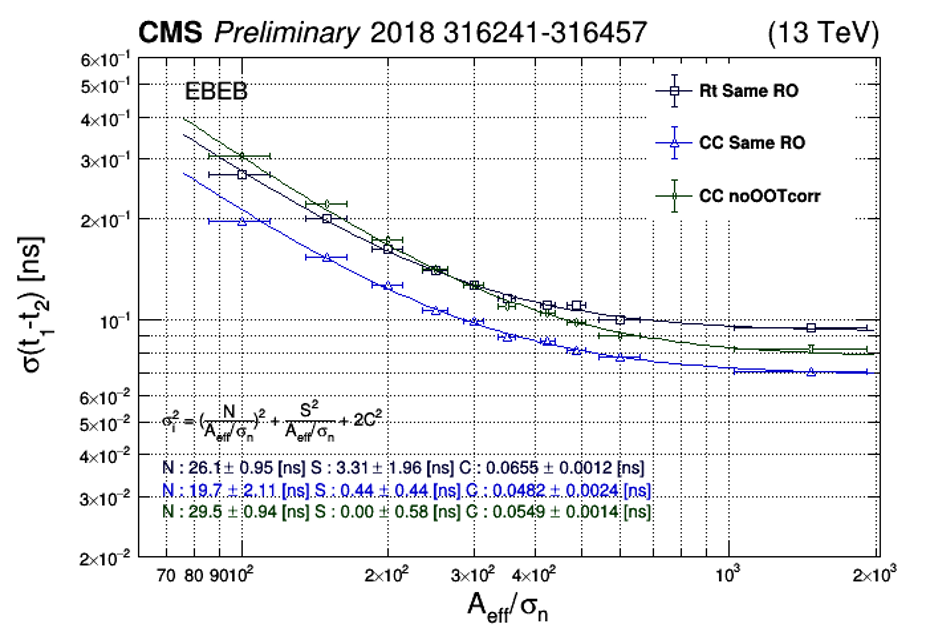
\includegraphics{fig/sec_gen/reso_w_wo_ootampcorr.png}}
%\caption{The Same RO unit time resolution for the ratio algorithm, the KUCC algorithm, and the KUCC algorithm without OOT amplitude corrections are plotted in runs 316241-316457 of Run 2018A. The resolutions are determined using the methods described in Section~\ref{sec:resmeth1}. It is seen that the resolution for the KUCC algorithm without OOT amplitude corrections is significantly degraded compared to the KUCC algorithm, as expected. The performance of the KUCC algorithm without OOT amplitude corrections is still noticeable improved when compared to the ratio method.}
%\label{cc_delay_res}
%\end{center}
%\end{figure}

%From this discussion it is clear that while the full KUCC time reconstruction with OOT amplitude corrections produces the best resolution for in time signatures, it is biased at large delay times. The full reconstruction is then optimal for use in cases involving predominately prompt physics. The KUCC time reconstruction without OOT amplitude corrections has no bias for delayed signatures but it does have a degraded resolution compared to the full reconstruction. The time reconstruction without OOT amplitude corrections is optimal for cases involving long lived particles and delayed time signatures. %\textcolor{red}{Given these observations, it is recommended that times for both the KUCC algorithm with OOT Amplitude corrections and without OOT Amplitude corrections are produced and saved.}